% This must be in the first 5 lines to tell arXiv to use pdfLaTeX, which is strongly recommended.
\pdfoutput=1
% In particular, the hyperref package requires pdfLaTeX in order to break URLs across lines.

\documentclass[11pt]{article}

% Remove the "review" option to generate the final version.
\usepackage[review]{acl}

% Standard package includes
\usepackage{times}
\usepackage{latexsym}
\usepackage[affil-it]{authblk}
\usepackage{graphicx}
\usepackage{subcaption}

% For proper rendering and hyphenation of words containing Latin characters (including in bib files)
\usepackage[T1]{fontenc}
% For Vietnamese characters
% \usepackage[T5]{fontenc}
% See https://www.latex-project.org/help/documentation/encguide.pdf for other character sets

% This assumes your files are encoded as UTF8
\usepackage[utf8]{inputenc}

% This is not strictly necessary, and may be commented out,
% but it will improve the layout of the manuscript,
% and will typically save some space.
\usepackage{microtype}

% If the title and author information does not fit in the area allocated, uncomment the following
%
%\setlength\titlebox{<dim>}
%
% and set <dim> to something 5cm or larger.

\begin{document}

% Add all figures used in the document.

\title{Cartoonifying Images and Videos}

\author{Ethan Fleming}
\affil{Portland State University, Winter 2022}

\maketitle

\begin{abstract}
  
  Image filters and transformations have been a popular and interesting avenue of image processing research for some time now.
  One small branch work offshooting from this involves producing cartoons from 3D models.
  Many of these methods require an artist to design a 3D model for the process though.
  Is it possible to generate cartoons or drawings from images and videos of natural 3D objects without making such models?
  This paper aims to investigate the possibilities of such a cartoonification process,
  ideally without having to use a large artificial intelligence framework.
  
\end{abstract}

\section{Introduction}

Art can be some of the most profitable work in existence, but also potentially one the most time-consuming.
Animation in particular can be dreadfully tedious for even the most passionate artists.
It doesn't help that animators must usually draw the original source frames at a much higher resolution than the scaled down final product.
Many recent efforts to reduce this time cost have involved rendering 3D models,
but this is computationally expensive and requires artists time to make all the 3D models and construct a scene and
then actors who are filmed by a team of camera people to create the best quality of animations for these 3D models.
(This is a process called "motion capture" or mocap for short).
And this is before one even gets to the topic of video editing!

This begs the question: is it possible to cut out the middle-person and just have the camera team and actors?
Can one cartoonify a live action source directly without needing all the hardware, 3D models, and artists?

\section{Method}

\subsection{K-means Clustering}

This paper primarily builds on an image compression algorithm developed by \citealp{WanXing}.

An image's file size is determined both by its resolution, but also by the variety of colors contained within it.
Therefore if one were to effectively reduce the image's color variance, its size would be scaled down.
For this application of K-means, the K centroids represent the set of K colors which best represent the image.
The result is an image where each pixel is the closest of those K colors to the original pixel, thus reducing the color variance drastically.

In the case of image compression, the idea is to find the lowest value of K such that the resulting compressed image still looks relatively the same.
In practice, low values of K usually result in a perturbed and potentially monochromatic image that differs significantly from the source.
Higher values of K are needed to maintain the original look of the source image, which can be computationally expensive.

However, the perturbations resulting from low values of K serve as the inspiration for this paper.
The optimum K to produce a cartoon is dependent on the source content's color complexity.
For cartoon generation, K needs to be high enough that the color profile of the source content is respected
(as too low a value results in monochromatic images), but also low enough that it doesn't feel too photorealistic.

\subsection{Canny Edge Detection}

Canny edge detection\footnote{\citep{Canny1986ACA}} is effective for finding clear lines in an image.
This is perfect for applying an outline to objects to an image to give it a drawing-like aesthetic.
For this application, one applies these lines after having reduced the color palette using K-means.

\subsubsection{Sobel-Feldman Operator}

Part of the Canny edge detection algorithm involves using a Sobel-Feldman operator\footnote{\citep{Sobel2014}} (another type of edge detection algorithm).
The resulting image after this operator is usually more noisy and not as clear and defined as that which Canny's produces.

For this paper the Sobel-Feldman operator is not suitable for the cartoon outlines,
but it is perfect for generating a mask to apply to the final cartoon's alpha channel.
This mask effectively texturizes the cartoon to add back some color variance which the K-means operation took away.

\subsection{Implementation}

The project associated with this paper was implemented using a Python 3 Anaconda environment.
It is dependent on Numpy, OpenCV, and Moviepy and was developed and tested using WSL Ubuntu 20.04.4 (LTS).

\section{Experiments}

\subsection{K-means tuning}

The first experiment involves tuning the K-means algorithm to best work for cartoon generation.
This is done by varying both the values of K, and the threshold constant.

\subsubsection{Varying values of K}

My first endeavor was to find the best values of K for cartoon generation.

\begin{figure}
  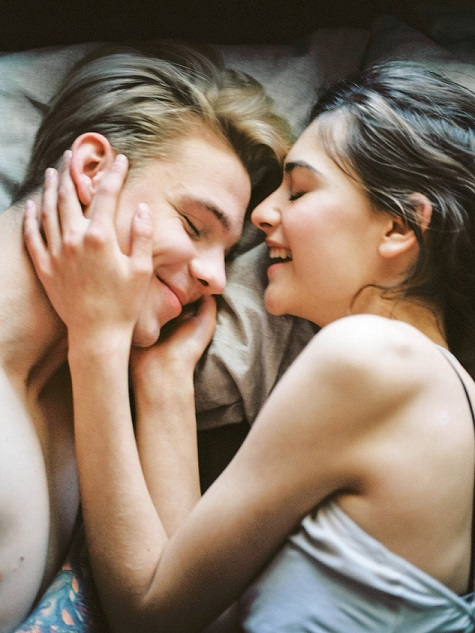
\includegraphics[width=\linewidth]{figures/pexels-photo-414032.jpeg}
  \caption{Original}
\end{figure}
\begin{figure}
  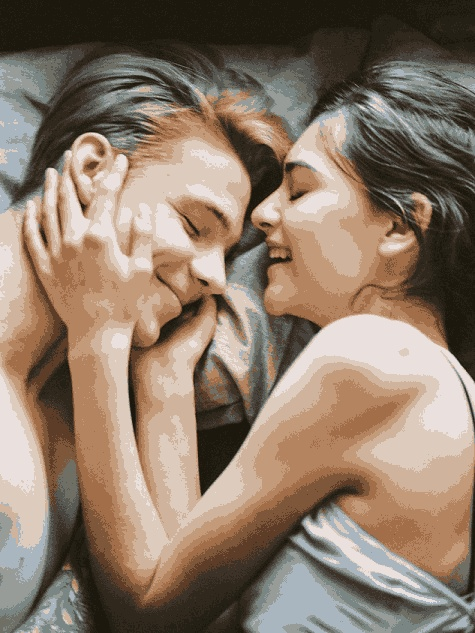
\includegraphics[width=\linewidth]{figures/lovers_K=18.jpg}
  \caption{K=18}
\end{figure}
\begin{figure}
  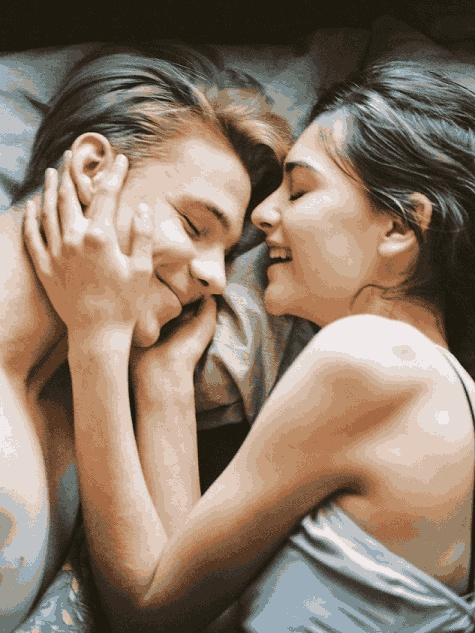
\includegraphics[width=\linewidth]{figures/lovers_K=24.jpg}
  \caption{K=24}
\end{figure}

Figures 1-3\footnote{Sourced from \url{https://images.pexels.com/photos/414032/pexels-photo-414032.jpeg}.}
demonstrate that generally K-values of 24 and higher start to look more photo-realistic.
The K should be tuned to specific source contents, but generally between 12 and 18 was best for cartoonification.

\subsubsection{Varying threshold values}

The threshold is defined as the point at which changes to the centroids are considered negligable.
Having a threshold value allows the algorithm to stop early, reducing compute cost.
The higher the threshold value, the sooner the algorithm determines the centroids are acceptable,
but threshold value too high will cause the colors to look inaccurate to the source image.
Very low thresholds on the other hand exponentiate compute cost (unless a maximum number of iterations is imposed).

\begin{figure}
  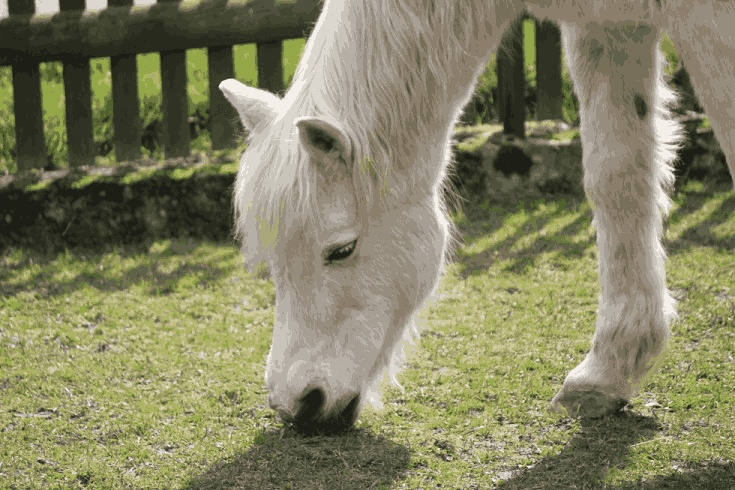
\includegraphics[width=\linewidth]{figures/white_horse_thresh=0.01.jpg}
  \caption{threshold = 0.01}
\end{figure}
\begin{figure}
  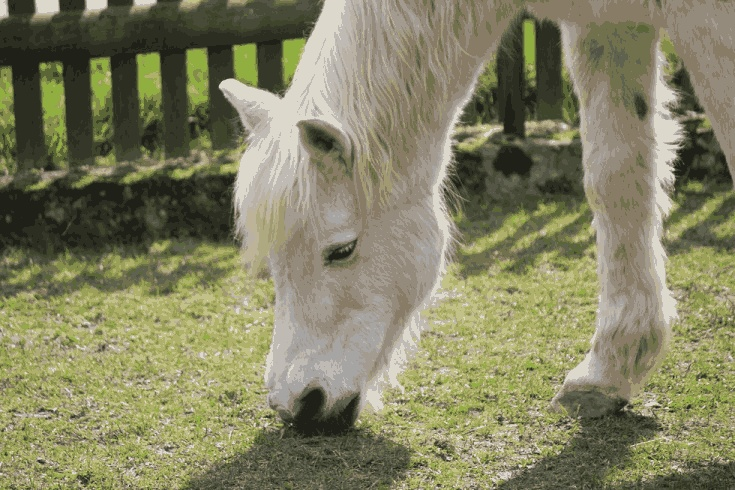
\includegraphics[width=\linewidth]{figures/white_horse_thresh=0.10.jpg}
  \caption{threshold = 0.10}
\end{figure}

The ideal threshold enlarges the images color patches without distorting or flattening the image beyond recognition.
Experimentation revealed that threshold values between 0.05 and 0.1 yielded the best cartoons,
which can be seen best in Figures 4 and 5\footnote{Sourced from \url{https://cc0.photo/wp-content/uploads/2022/02/White-shaggy-horse-grazes-in-the-meadow-980x653.jpg}.}.

\subsection{Canny edge tuning}

Tuning the canny edge detection algorithm primarily involved changing the size of the Gaussian kernel filter applied to the image.
Smaller kernels produce less blurring and therefore more detail (which is in this case referring to the number of lines detected),
whereas larger kernels blur the image and remove detail.

\begin{figure}
  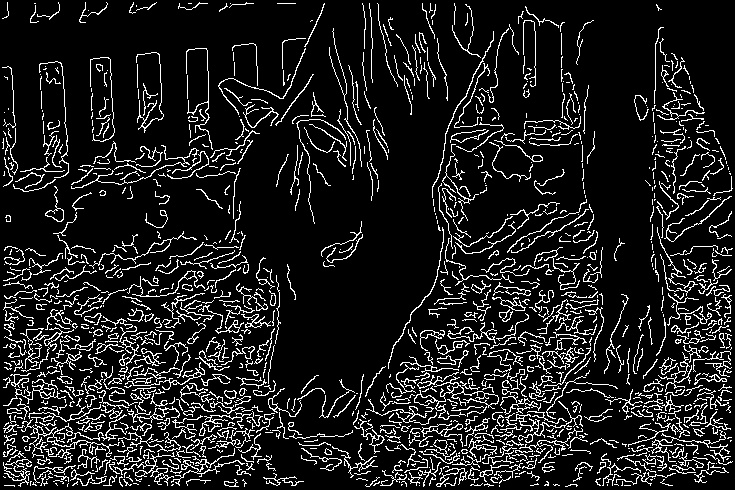
\includegraphics[width=\linewidth]{figures/white_horse_ksize=5.jpg}
  \caption{kernel size = 5}
\end{figure}

\begin{figure}
  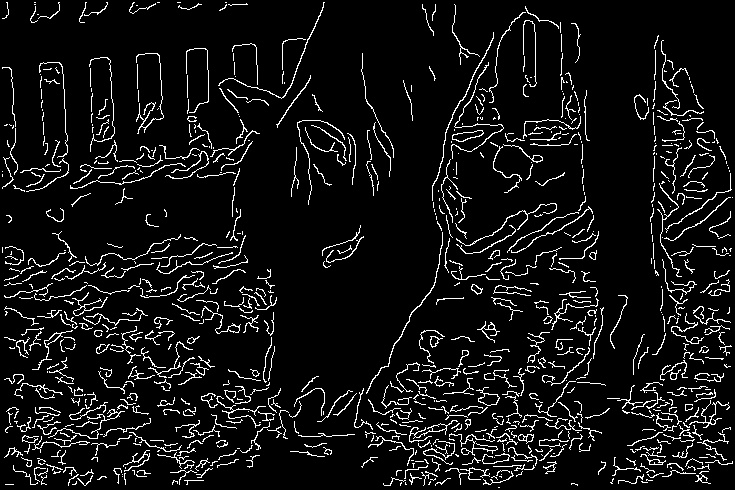
\includegraphics[width=\linewidth]{figures/white_horse_ksize=7.jpg}
  \caption{kernel size = 7}
\end{figure}

\begin{figure}
  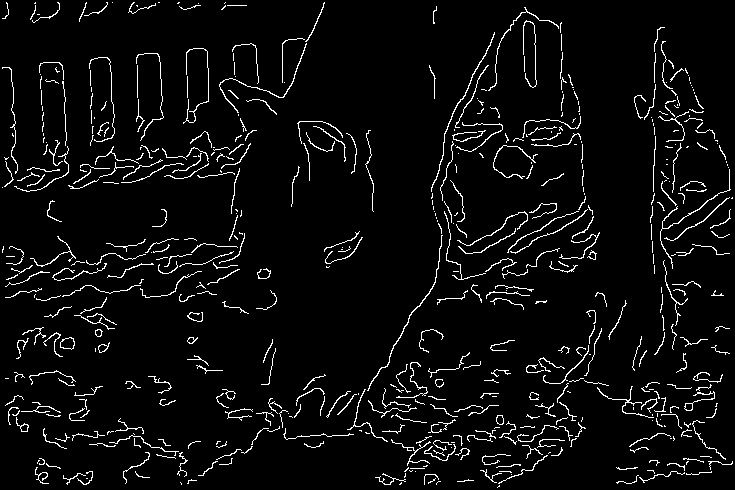
\includegraphics[width=\linewidth]{figures/white_horse_ksize=9.jpg}
  \caption{kernel size = 9}
\end{figure}

Experimentation showed that kernel sizes between 5 and 9 worked best, with 7 being a general optimum.
This is shown in Figures 6-8.

\section{Results}

Figures 9 and after are some of the results of the entire cartoonification process.
\begin{figure}
  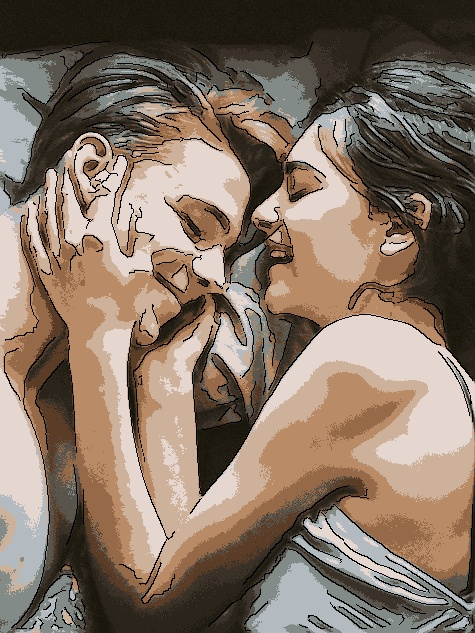
\includegraphics[width=\linewidth]{figures/lovers_K=12_ksize=7.jpg}
  \caption{K = 12, kernel size = 7}
\end{figure}

\begin{figure}
  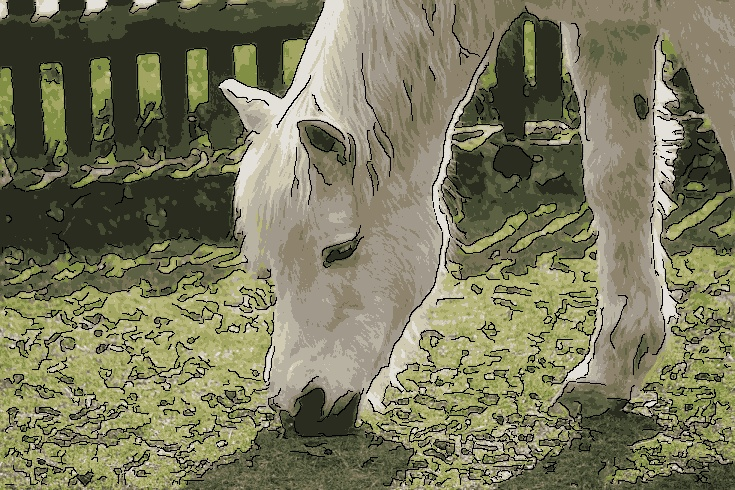
\includegraphics[width=\linewidth]{figures/white_horse_K=12_ksize=7.jpg}
  \caption{K = 12, kernel size = 7}
\end{figure}

\begin{figure}
  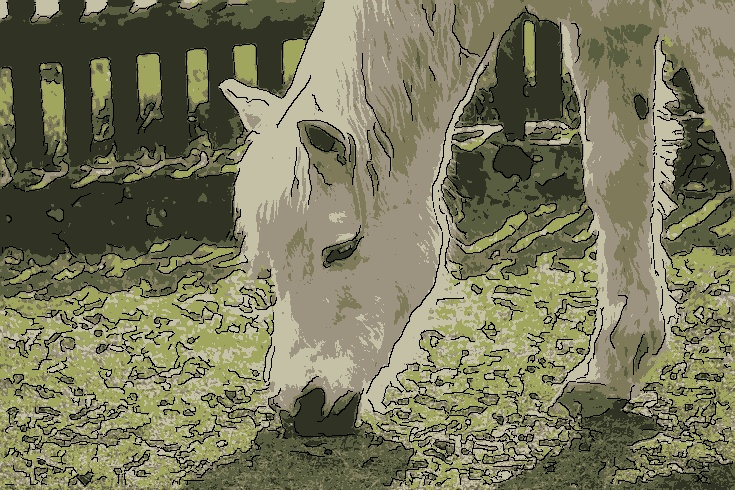
\includegraphics[width=\linewidth]{figures/white_horse_K=6_ksize=7.jpg}
  \caption{K = 6, kernel size = 7}
\end{figure}

\subsection{Videos}

The project implemented for this paper is capable of applying this cartoonification process to the frames of a video.
This can take a long time, but does not use that much memory or compute power.

\section{Conclusion}

Does the algorithm make photos look like drawings or cartoons?
Not really, but the style produced is intriguing.
Though definitely ot enough to motivate people to pursue this as a media format.

Perhaps artists might be able to use this to make a baseline set of frames which they can paint over?
If so, that could substantially reduce the time it takes them to animate each frame.

\section {Future Work}

When it comes to videos, performance of this algorithm is paramount.
Significant refactoring to optimize and parallelize this code is necessary.

Additionally, the colors of a particular object change over the course of a video.
Perhaps the K-means should find a set of centroids for all the frames rather than each individually?
This way each object might retain the same set of colors throughout a video.

Lastly, instead of being manually tuned, some of the hyperparameters could be made to be programmatically determined.
The algorithm could find an optimum K based on an image/frame's color complexity,
and an optimum kernel size potentially by detecting the number of features in the background vs the foreground
and adjusting accordingly.

% Entries for the entire Anthology, followed by custom entries
\bibliography{bibliography}

\end{document}
